\documentclass[hyperref={dvipdfmx,pdfpagelabels=false}]{beamer}
\title{Einführung in Matlab - Einheit 5}
\subtitle{Numerische Mathematik}
\mode<article>
{
  \usepackage{fullpage}
  \usepackage{pgf}
  \usepackage{hyperref}
  \setjobnamebeamerversion{beamer}
}

\mode<presentation>
{
  %\usetheme{Frankfurt}
 %\usetheme{My}
  \usetheme{Madrid}
  % or ...
%\usecolortheme{seagull}
  %\setbeamercovered{transparent}
  %\setbeamercovered{dynamic}
  % or whatever (possibly just delete it)
}
\usenavigationsymbolstemplate{}
\usefonttheme{structurebold}
\usepackage{multimedia}
\usepackage{tikz}
\usepackage{fontspec,xunicode,xltxtra}
%\usepackage[scaled=.90]{helvet}
% Or whatever. Note that the encoding and the font should match. If T1
% does not look nice, try deleting the line with the fontenc.

\setbeamertemplate{footline}
{
\leavevmode
%\hbox{\begin{beamercolorbox}[wd=.5\paperwidth,ht=2.5ex,dp=1.125ex,
%leftskip=.3cm plus1fill,rightskip=.3cm]{author in head/foot}%
%    \usebeamerfont{author in head/foot}\insertshortauthor
%  \end{beamercolorbox}%
%  \begin{beamercolorbox}[wd=.5\paperwidth,ht=2.5ex,dp=1.125ex,leftskip=.3cm,
%rightskip=.3cm plus1fil]{title in head/foot}%
%    \usebeamerfont{title in head/foot}\insertshorttitle\hfill

\hfill\insertframenumber  \hspace{3pt}

%\inserttotalframenumber
%\hspace*{2ex}
%  \end{beamercolorbox}}%
  \vskip3pt%
}

%\usepackage[english]{babel}
\usepackage[ngerman]{babel}
\selectlanguage{ngerman}

%
% math/symbols
%
\usepackage{amssymb}
\usepackage{amsthm}
% \usepackage{latexsym}
\usepackage{amsmath}
%\usepackage{listings}
\usepackage[framed]{mcode}
%\usepackage{mcode}

\usepackage{mydef}
\usepackage{cmap} % you can search in the pdf for umlauts and ligatures
%\usepackage{colonequals} %corrects the definition-symbols \colonequals (besides others)
\title{Einführung in Matlab}
%
%\subtitle{Disputation} % (optional)

\author{Jochen Schulz}
% - Use the \inst{?} command only if the authors have different
%   affiliation.

\institute{Georg-August Universit\"at G\"ottingen \pgfimage[height=0.5cm]{../figures/unilogo3}}
% - Use the \inst command only if there are several affiliations.
% - Keep it simple, no one is interested in your street address.

\date{\today}

\subject{Einführung in Matlab}
% This is only inserted into the PDF information catalog. Can be left
% out. 



% If you have a file called "university-logo-filename.xxx", where xxx
% is a graphic format that can be processed by latex or pdflatex,
% resp., then you can add a logo as follows:

%\logo{\pgfimage[height=0.5cm]{figures/unilogo3}}


% Delete this, if you do not want the table of contents to pop up at
% the beginning of each subsection:
% \AtBeginSubsection[]
% {
%   \begin{frame}<beamer>
%     \frametitle{Aufbau}
%     \tableofcontents[currentsection,currentsubsection]
%   \end{frame}
% }

\AtBeginSection[]
{
  \begin{frame}<beamer>
    \frametitle{Aufbau}
    \tableofcontents[currentsection,currentsubsection]
  \end{frame}
}


\begin{document}



\maketitle

\section{Numerische Mathematik}

\subsection{Poisson Problem}
%
% Slide
% 
\begin{frame}[fragile]\frametitle{Poisson Problem}
\begin{itemize}
\item Poisson Problem beschreibt station\"are W\"armeverteilungen.
\item {\it Poisson Problem:} Suche  $u \in
C^2(\Omega)\cap C(\overline{\Omega})$ mit
\[
\left \{ \begin{array}{rcll}
- \triangle u & = & f & \mbox{in } \Omega\\
u & = & 0 & \mbox{auf } \partial \Omega\\ 
\end{array} \right.
\]
f\"ur $\Omega=(0,1)^2$ und $f \in C(\Omega)$.
\item  {\it Laplace-Operator} 
$ \triangle u := \sum_{i=1}^d \frac{\partial ^2 u}{\partial x_i^2} $
\end{itemize}
\end{frame}
%
% Slide
% 
\begin{frame}[fragile]\frametitle{Diskretisierung}
\begin{itemize}
\item \"Aquidistante Gitterweite $h= \frac 1 N$,
$N \in \mathbb{N}$
\item Menge aller Gitterpunkte 
\[ Z_h := \left\{ (x,y) \in \overline{\Omega} \ \mid \ x=z_1h, \ y=z_2h \text{ mit }
z_1,z_2 \in \mathbb{Z} \right\}. \]
\item Innere Gitterpunkte: $\omega_h := Z_h \cap \Omega$
\end{itemize}
\end{frame}
%
% Slide
% 
\begin{frame}[fragile]\frametitle{Diskretisierung}
\begin{itemize}
\item Approximation von $ \frac{\partial ^2 u}{\partial
  x^2} (x,y)$
{\small \[ \frac{u(x -h,y) - 2 u(x,y) + u(x+h,y)}{h^2} = \frac{\partial ^2 u}{\partial
  x^2} (x,y) + \mathcal{O}(h^2) \]}
\item  Approximation von $ \frac{\partial ^2 u}{\partial
  y^2} (x,y)$
{\small \[ \frac{u(x ,y-h) - 2 u(x,y) + u(x,y+h)}{h^2} = \frac{\partial ^2 u}{\partial
  y^2} (x,y) + \mathcal{O}(h^2) \]}
\item Addition ergibt f\"ur $ \triangle u(x,y)$ die N\"aherung
{\footnotesize \[
 \frac{1}{h^2} \left( u(x,y-h) + u(x-h,y) - 4 u(x,y) + u(x,y+h) +
 u(x+h,y)  \right) 
\] }
\end{itemize}
\end{frame}
%
% Slide
% 
\begin{frame}[fragile]\frametitle{Diskretisierung}
\begin{itemize}
\item Definition $u_{i,j}:=u(ih,jh)$ ergibt an Gitterpunkten $(ih,jh)$
\[ -u_{i,j-1} - u_{i-1,j} + 4 u_{i,j} - u_{i+1,j} - u_{i,j+1} = h^2 f_{ij} \] 
mit $i,j \in \{ 1, \dots , N-1 \}$ und $f_{ij}:=f(ih,jh)$. 
\item Randbedingungen ergeben
$u_{0,i}=u_{N,i}=u_{i,0}=u_{i,N}=0$, $i=0, \dots ,N$.
\end{itemize}
\end{frame}

%
% Slide
% 
\begin{frame}[fragile]\frametitle{Diskretisierung}
\begin{itemize}
\item Lexikografische Sortierung der inneren Unbekannten 
{\small \[ \begin{array}{cccc}
(h,(N-1)h) & (2h,(N-1)h) & \hdots & ((N-1)h,(N-1)h)\\
\vdots & \vdots & \vdots & \vdots \\
(h,2h) & (2h,2h) & \hdots & ((N-1)h,2h)\\
(h,h), & (2h,h) & \hdots & ((N-1)h,h)\\
\end{array} \]
}
ergibt Vektor $U_{i+(N-1)(j-1)}=u_{i,j}$.
\end{itemize}
\end{frame}
%
% Slide
% 
\begin{frame}[fragile]\frametitle{Diskretisierung}
Lineares Gleichungssystem f\"ur $U=(U_i)_{i=1}^{(N-1)^2}$
\[ A U = F \]
mit 
\begin{itemize}
\item $F:=(f_i)_{i=1}^{(N-1)^2}$ mit $f_{i+(N-1)(j-1)}=f(ih,jh)$, $i,j \in \{1,
\dots ,N-1 \}$,
\item  \begin{eqnarray*} 
A & := & \frac{1}{h^2} tridiag(-I_{N-1}, T, -I_{N-1}) \in \mathbb{R}^{(N-1)^2
 \times (N-1)^2},\\
 T & := & tridiag(-1,4,-1) \in \mathbb{R}^{(N-1)\times (N-1)}. 
\end{eqnarray*}
\end{itemize}
\end{frame}
%
% Slide
% 
\begin{frame}[fragile]\frametitle{Implementierung}
\begin{lstlisting}
function loes = poisson (f,n)
f = fcnchk(f);
A = gallery('poisson',n-1); 
% Erzeuge rechte Seite und Mesh
mesh = zeros(2,(n-1)^2);
F = zeros((n-1)^2,1);
for i = 1:(n-1)
    for j = 1:(n-1)
        F(i+(n-1)*(j-1)) = (1/n)^2*f(i/n,j/n);
        loes.mesh(:,i+(n-1)*(j-1)) = [i/n; j/n]; 
    end
end
% Loese das lineare System
loes.x = A \ F;
\end{lstlisting}
\end{frame}
%
% Slide
% 
\begin{frame}[fragile]\frametitle{Implementierung}
\begin{lstlisting}

% Ergaenze Randbedingungen
loes.x = [ loes.x; zeros(4*(n+1),1)];
loes.mesh = [loes.mesh, [zeros(1,n+1); 0:1/n:1]];
loes.mesh = [loes.mesh, [ones(1,n+1);  0:1/n:1]];
loes.mesh = [loes.mesh, [0:1/n:1; ones(1,n+1)]];
loes.mesh = [loes.mesh, [0:1/n:1; zeros(1,n+1)]];

% Plotten
plot3(loes.mesh(1,:),loes.mesh(2,:),loes.x,'*');
figure;
[X,Y] = meshgrid(0:1/n:1,0:1/n:1);
Fi = TriScatteredInterp(loes.mesh(1,:)', loes.mesh(2,:)',loes.x,'linear');
Z = Fi(X,Y);
surf(X,Y,Z);
\end{lstlisting}
\end{frame}

\subsection{Differentialgleichungen}
%
% Slide
%
\begin{frame}[fragile]\frametitle{Gew\"ohnliche Differentialgleichungen}
Sei $I \subset \mathbb{R}$ ein Intervall. Bei einer gewöhnlichen Dgl. sucht man eine Funktion $y:I \
\longrightarrow \mathbb{R}^n$, so dass
\alert{ \[ \frac{d}{dt}y(t)=f(t,y(t)), t\in I\quad y(t_0)=y_0, \]}
wobei $y_0 \in \mathbb{R}^n$ ein vorgegebener Anfangswert an $t_0\in I$
und $f:I \times \mathbb{R}^n \longrightarrow \mathbb{R}^n$ die
rechte Seite ist. Au{\ss}erdem sei $ \frac{d}{dt}y(t) :=(\frac{\partial
  y_1(t)}{\partial t}, \dots, \frac{\partial
  y_n(t)}{\partial t})^t$. \\
\alert{Beispiele:}\\
{\scriptsize
$\frac{d}{dt} y(t) = y(t), \ y(t_0)=y_0$, \quad L\"osung:
$y(t)=y_0 e^{t-t_0}$\\
$\frac{d}{dt} y(t) = e^y \sin(t)$, \quad L\"osung: $y(t)=-\log( \cos(x)+C)$, $C+\cos(x)>0$ }
\end{frame}
%
% Slide
%
\begin{frame}[fragile]\frametitle{Skalares Beispiel}
L\"ose f\"ur $0 \leq t \leq 3$ mit \alert{ ode45} die Dgl.
\alert{ \[ \frac{d}{dt} y(t) = -y(t)-5e^{-t}\sin5t, \quad y(0)=1. \]}
\begin{itemize}
\item Die rechte Seite als eigene Funktion:
\begin{lstlisting}
function z = rechte_seite1(t,y)
% rechte_seite1   ODE Beispiel
%         z=rechte_seite1(t,y)
z = -y-5*exp(-t)*sin(5*t);
\end{lstlisting}
\end{itemize}
\end{frame}
%
% Slide
%
\begin{frame}[fragile]\frametitle{Skalares Beispiel}
\begin{itemize}
\item Ausrechnen und Plotten
\begin{lstlisting}
tspan = [0,3]; aw = 1;
[t,y] = ode45(@rechte_seite1,tspan,aw);
plot(t,y,'*--','Linewidth',3)
xlabel('t'), ylabel('y(t)')
\end{lstlisting}
\end{itemize}
\begin{center}
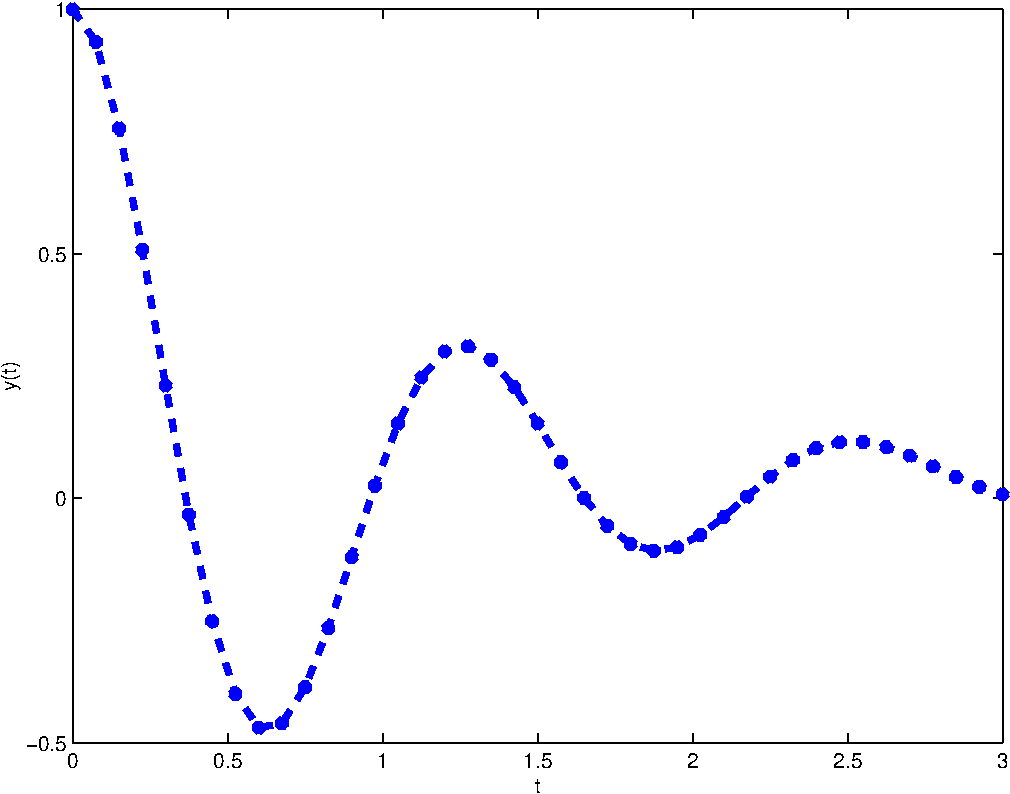
\includegraphics[width=0.5\textwidth]{./figures/loesung_dgl1} 
\end{center}
\end{frame}
%
% Slide
%
\begin{frame}[fragile]\frametitle{ODE in MATLAB} 
\begin{lstlisting}
[<t>,<y>] = ode45(<@fun>, <tspan>, <aw>, <options>)
\end{lstlisting}
\begin{itemize}
\item \mcode{@fun} steht f\"ur die rechte Seite der Dgl. (m-File).
\item $aw \in \mathbb{R}^n$ ist der Anfangswert.
\item $tspan$ gibt das Zeitintervall an, auf dem die Dgl. berechnet
  werden soll. Normalerweise ist es von der Form
  \mcode{tspan=[t_0, t_1]}. Dann wird die Dgl. auf dem Intervall $[t_0,
  t_1]$ berechnet (Anfangswert: $y(t_0)=aw$).
\item Rückgabewerte: Vektoren $t$ und Matrizen $y$. Dabei ist
  $y(:,i)$ die L\"osung an der Stelle $t(i)$. Die Punkte $t_i$ werden
  automatisch bestimmt.
\item Durch die optionale Angabe von \mcode{options} kann der L\"oser
  gezielt eingestellt werden. 
\item Spezifiziert man mehr als zwei Zeitpunkte in \mcode{tspan}, so gibt MATLAB die
  L\"osung genau an diesen Zeitschritten zur\"uck.
\end{itemize}
\end{frame}
%
% Slide
%
\begin{frame}[fragile]\frametitle{Optionen}
Die genauen Parameter der ODE-L\"oser k\"onnen durch\\

\begin{lstlisting}
options = odeset('Eigenschaft 1','Spez. 1',...
  'Eigenschaft 2','Spez. 2',...) 
\end{lstlisting}

gesteuert werden. Die wichtigsten Parameter sind \mcode{AbsTol}
(Default $10^{-6}$) und \mcode{RelTol} (Default: $10^{-3}$). \\[0.5cm]
\alert{Beispiel:}
\begin{lstlisting}
options = odeset('AbsTol',1e-7,'RelTol',1e-4)
\end{lstlisting}
\end{frame}
%
% Slide
%
\begin{frame}[fragile]\frametitle{Andere L\"oser}
\begin{tabular}{ccp{5.5cm}c}
\hline
L\"oser & Steifigkeit & Algorithmus & Ordnungen\\
\hline
\mcode{ode45} & nicht steif & Expliziter Runge-Kutta L\"oser &  4, 5 \\
\mcode{ode23} & nicht steif & Expliziter Runge-Kutta L\"oser &  2, 3 \\
\mcode{ode113} & nicht steif & Explizites Mehrschrittverfahren & 1 - 13\\
\mcode{ode15s} & steif & Implizites Mehrschrittverfahren& 1 - 5\\
\mcode{ode23s} & steif &Modifiziertes Rosenbrockverfahren& 2, 3\\
\mcode{ode23t} & mittel steif & implizite Trapez Regel& 2, 3\\
\mcode{ode23tb} & steif & Implizites Runge-Kutta Verf.& 2, 3\\
\end{tabular}
%Ein lineares DG System mit konstanten Koeffizienten heißt steif, wenn
%seine Eigenwerte alle negativen Realteil besitzen und sein Steifigkeitsquotient
%groß ist.
%Sei µ1 der betragsgrößte und µ2 der betragskleinste Realteil der Eigenwerte einer Jacobi-Matrix, 
%dann wird der Steifigkeitsquotient q dieser Matrix definiert durch:
%q = µ1/µ2
\end{frame}

\subsection{Lorenz-Gleichungen}
%
% Slide
%
\begin{frame}[fragile]\frametitle{Die Lorenz-Gleichungen}
\begin{itemize}
 \item Chaostheorie / Schmetterlingseffekt.
\end{itemize}

\begin{eqnarray*}
\frac{d}{dt} y_1(t) & = & 10 (y_2(t) -y_1(t)) \\
\frac{d}{dt} y_2(t) & = & 28 y_1(t) -y_2(t) -y_1(t)y_3(t)\\ 
\frac{d}{dt} y_3(t) & = & y_1(t)y_2(t) -8y_3(t)/3
\end{eqnarray*}


rechte Seite:
\begin{lstlisting}
function z = lorenz_rechte_seite(t,y)
z = [10*(y(2)-y(1));...
    28*y(1)-y(2)-y(1)*y(3);...
    y(1)*y(2)-8*y(3)/3];
\end{lstlisting}
\end{frame}
%
% Slide
%
\begin{frame}[fragile]\frametitle{Die Lorenz-Gleichungen}
\begin{lstlisting}
%---------------------------------
%   lorenz_gl.m
%  Eine Approximation der Lorenzgleichungen
%-----------------------------------------
tspan = [0,30]; aw = [0;1;0];
options = odeset ('AbsTol',1e-7,'RelTol',1e-4);
[t,y] = ode45(@lorenz_rechte_seite,tspan,aw, options);

subplot(2,2,1),plot3(y(:,1),y(:,2),y(:,3)), 
subplot(2,2,2),plot(y(:,1),y(:,2)),xlabel('y_1'),ylabel('y_2');
subplot(2,2,3),plot(y(:,1),y(:,3)),xlabel('y_1'),ylabel('y_3');
subplot(2,2,4),plot(y(:,2),y(:,3)),xlabel('y_2'),ylabel('y_3');
\end{lstlisting}
\end{frame}
%
% Slide
%
\begin{frame}[fragile]\frametitle{Die Lorenz-Gleichungen}
\begin{center}

\includegraphics[width=0.8\textwidth]{./figures/lorenz}
\end{center}
\end{frame}

\end{document}